\documentclass[12pt,opeany,a4paper,twoside]{book}   

\usepackage[czech]{babel}
\usepackage[utf8]{inputenc}
% Nedeli slova pomlckou
\usepackage[none]{hyphenat}
% URL odkazy a zalamovani
\PassOptionsToPackage{hyphens}{url}
% Odkazy v obsahu nejsou zvyraznene
\usepackage[hidelinks]{hyperref}
% Obrazky
\usepackage{graphicx}
% Odstrani kapitoly
\usepackage{titlesec}
% Okraje
\usepackage[margin=2.5cm]{geometry}
% Pro justify zarovnani
\usepackage{ragged2e}
% Radkovani
\renewcommand{\baselinestretch}{1.5} 
% Times New Roman
\usepackage{times}
% PDF logo
\usepackage{pdfpages}

\author{Petr Michalík, O8.A\\Gymnázium, Praha 6, Nad Alejí 1952}
\title{Aplikace pro generování a ověřování jednorázových hesel}
\date{2016/2017}

% Nastaveni pro hyperlink
\hypersetup{
    bookmarks=false,         % show bookmarks bar?
    unicode=true,          % non-Latin characters in Acrobat’s bookmarks
    pdftoolbar=true,        % show Acrobat’s toolbar?
    pdfmenubar=true,        % show Acrobat’s menu?
    pdffitwindow=true,     % window fit to page when opened
    pdfstartview={Fit},    % fits the width of the page to the window
    pdftitle={Aplikace pro generování a ověřování jednorázových hesel},    % title
    pdfauthor={Petr Michalík  \\ Gymnázium, Praha 6, Nad Alejí 1952 },     % author
}

% Odstrani hlavicky stranky
\pagestyle{empty}
% Odstrani automaticke vkladani prazdne stranky
\let\cleardoublepage\clearpage
% Odstrani kapitoly
\titleformat{\chapter}{\normalfont\huge}{\thechapter.}{24pt}{\huge\it}
%Odstrani presahujici slova
\sloppy
\begin{document}

%\maketitle
%**********************************************************************
\begin{titlepage}
	\centering	
	{~\par}
	\vspace{4cm}
	{\scshape\LARGE  Maturitní práce  \par}
	\vspace{1cm}
	{\huge\bfseries Aplikace pro generování a ověřování jednorázových hesel \par}
	\vspace{1cm}
	{\large Uživatelská příručka \par}
	\vspace{4cm}
	
	\vfill
	
% Bottom of the page
	{\large Petr Michalík \par}
	{\large Gymnázium, Praha 6, Nad Alejí 1952 \par}
	{\large 2016/2017\par}
\end{titlepage}

% Cisluje i titlulni stranu
\pagestyle{plain}
\setcounter{page}{2}
% Zarovnani do bloku
\justify
%**********************************************************************
{\normalfont\huge Prohlášení}
\vspace{2cm}

\raggedright
Prohlašuji, že jsem na maturitním projektu pracoval samostatně pouze za pomoci uvedených zdrojů.
\\
\vfill
{V Praze \today}
\\
\raggedleft {\it Podpis }
\clearpage
%**********************************************
\shorthandoff{-}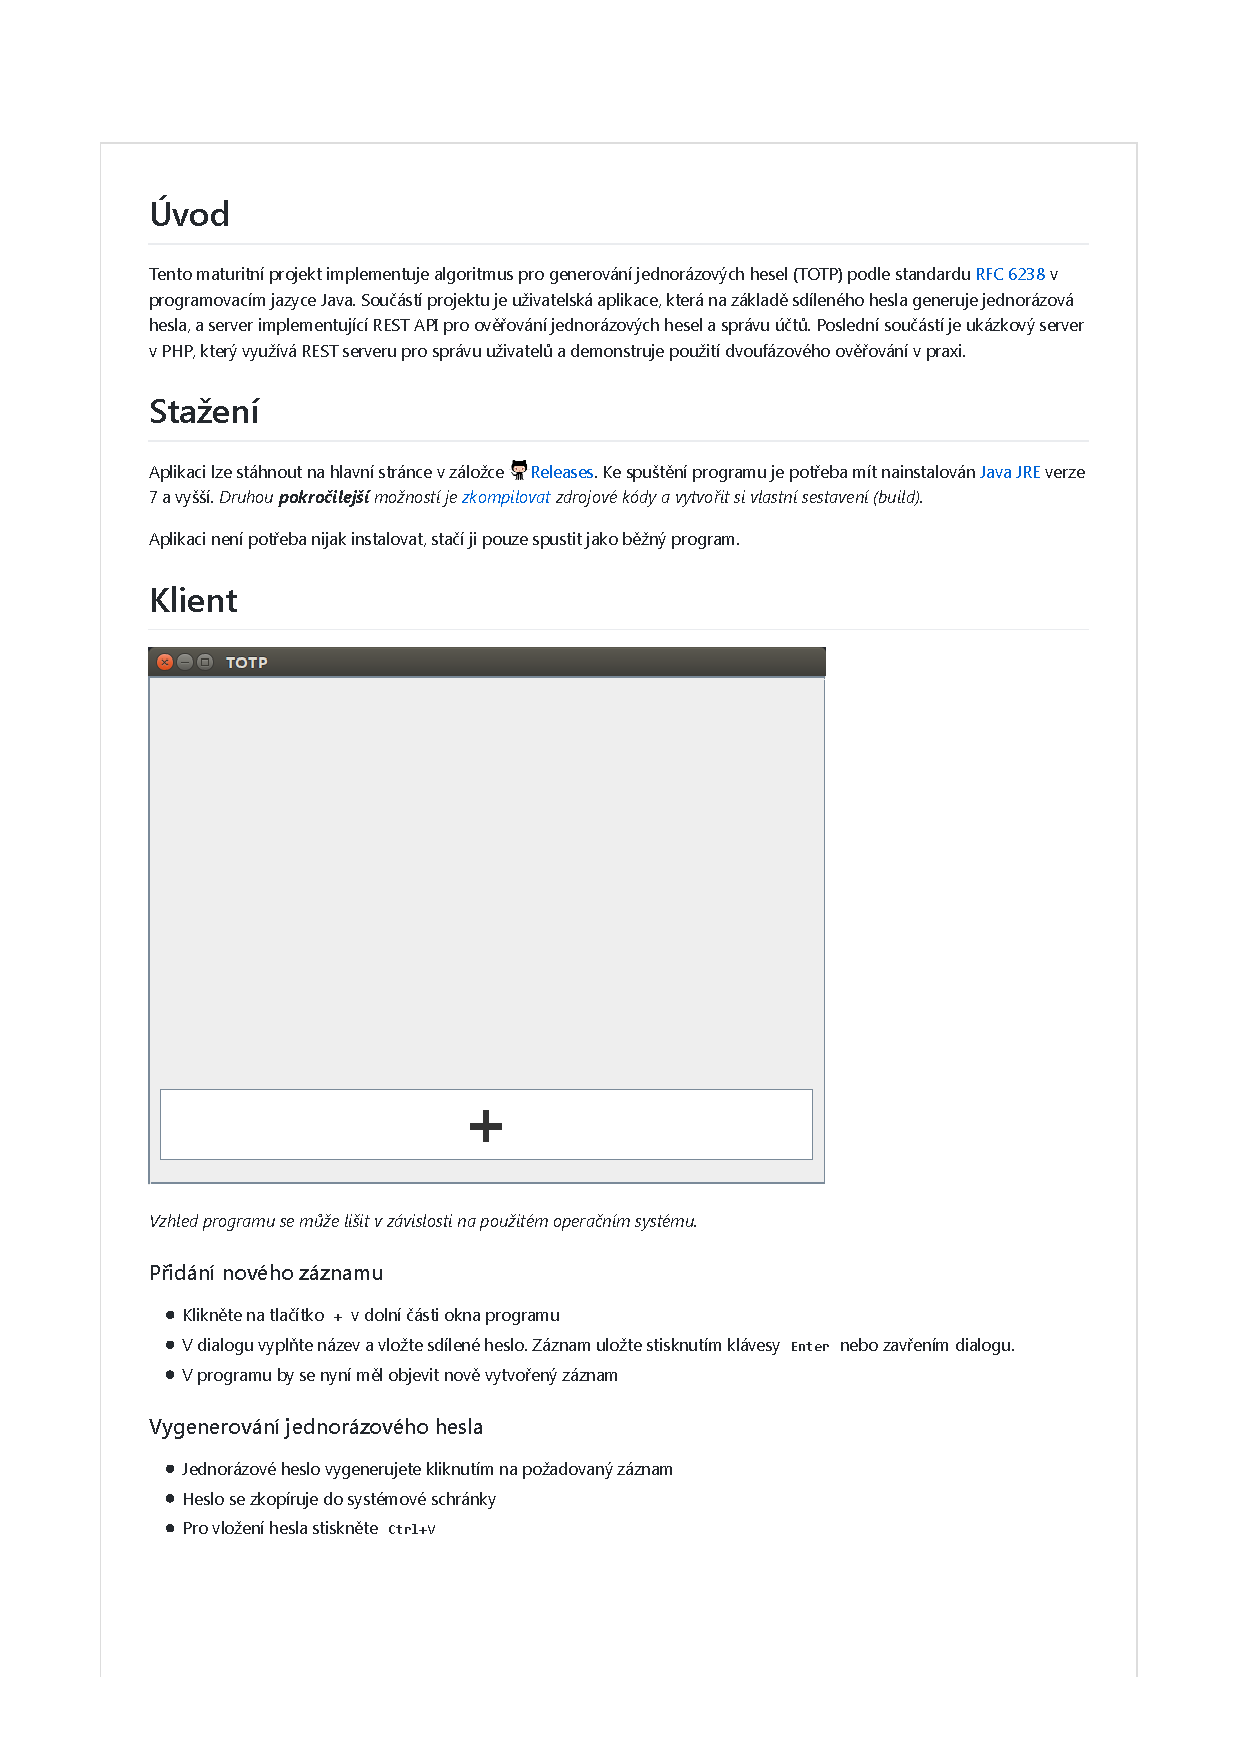
\includepdf[pages=-]{prirucka.pdf}\shorthandon{-}
%**********************************************
\justify
{\normalfont\huge Zdroje a knihovny}
\vspace{2cm}

\begin{itemize}
\item RFC 6238 (TOTP standard), \url{https://tools.ietf.org/html/rfc6238}
\item RFC 4226 (HOTP standard), \url{https://tools.ietf.org/html/rfc4226}
\item jUnit, \url{http://junit.org/}
\item Hamcrest, \url{http://hamcrest.org/}
\item Apache Commons Codec, \url{https://commons.apache.org/proper/commons-codec/}
\item Restlet, \url{https://restlet.com/open-source/}
\item JSON-simple, \url{https://code.google.com/archive/p/json-simple/}
\end{itemize}

\end{document}